% !Mode:: "TeX:UTF-8"

\chapter{可见光多波段通信系统概述}
\section{引言}
得益于LED灯在照明市场的风行,能使LED灯兼顾通信和照明两重功能的可见光通信技术因其绿色环保、高速便捷、频谱资源不受限制等优点受到了越来越多的关注。可见光通信技术极有可能在未来的无线通信中占有一席之地,特别是诸如机舱、医院和矿井这些特殊应用场景下。本章将先介绍可见光通信的基本原理,包括基础硬件发光二极管(LED)和光电二极管(PD)的基本工作原理及可见光通信系统模型,然后将概述OFDM在可见光通信中的应用,并且比较ACO-OFDM及DCO-OFDM之间的区别,最后将简介自适应传输技术及其在可见光通信中的应用。
\section{室内可见光通信基本原理}
\subsection{可见光系统模型}
\begin{figure}[htbp]
\centering
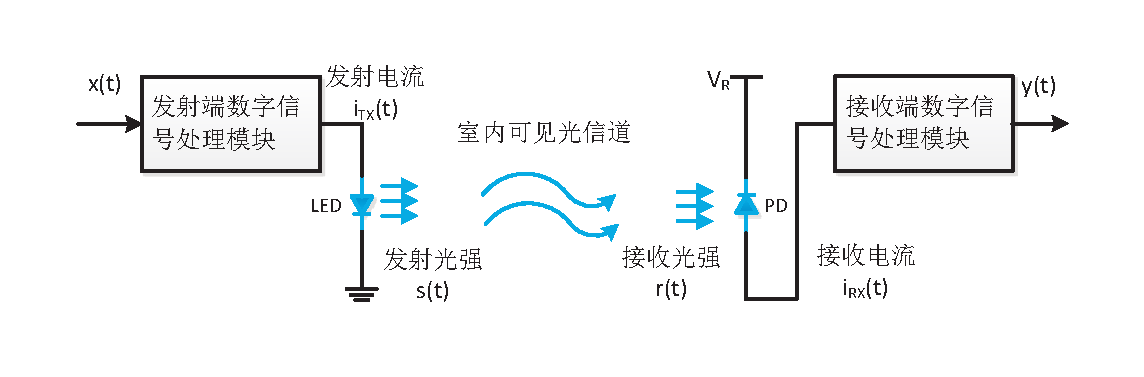
\includegraphics[width=\textwidth]{figures/Chapter-2/BasicOpticalSystem.eps}
\caption{光无线通信系统模型}
\label{fig:BasicOpticalSystem}
\end{figure}
\subsection{光电元器件简介}
\subsubsection{发光二极管(LED)}
\subsubsection{光电二极管(PD)}

\section{OFDM技术在室内可见光通信中的应用}
\subsection{OFDM技术简介}
\subsection{可见光中的OFDM调制}
\section{自适应传输技术简介}
\section{本章小结}
